\chapter{\label{chap:spelunkbots}SpelunkBots}
Em 2014, Daniel Scales e Thomas Thompson, da Universidade de Derby no Reino
Unido, criaram o \textit{SpelunkBots}\cite{SPELUNKBOTSPAPER}, um
\textit{framework} que permite a programação de \textit{bots} para o jogo
Spelunky. Um dos objetivos dos criadores é utilizar a aplicação para criar uma
competição de inteligência artificial para o jogo. O \textit{framework} foi
desenvolvido utilizando uma combinação do código-fonte original do jogo
\textit{Spelunky} -- distribuído gratuítamente no \textit{website}
oficial\footnote{http://www.spelunkyworld.com/original.htm} --, o motor de
criação de jogos \textit{GameMaker} e uma solução \textit{DLL} programada com a
linguagem C++.


%----------
\section{Modo de Uso}
Apesar de possuir acesso irrestrito ao código-fonte de \textit{Spelunky}, os
autores reconheceram que a linguagem de programação \textit{GML}, nativa do
motor \textit{GameMaker}, não é a escolha ideal para realizar a programação de
uma inteligência artificial complexa. A \textit{GML} foi criada com o intuito de
fornecer a desenvolvedores de jogos iniciantes uma maneira fácil e rápida de
programar jogos, mas não é a melhor escolha para programadores mais experientes,
pois requer que o desenvolvedor se adeque ao \textit{GameMaker} -- os arquivos
de código em \textit{GML} só podem ser editados de dentro do motor -- e a uma
linguagem de programação nova.

Sabendo que o \textit{GameMaker} é capaz de executar código externo através de
\textit{Dynamic-link Libraries} (\textit{DLLS}), os autores desenvolveram um
projeto em C++ que gera uma solução no formato \textit{DLL} para permitir que os
usuários possam programar \textit{bots} utilizando a linguagem de programação
C++. Para programar em C++, portanto,  é necessário fazer uso de uma ferramenta de
compilação externa para gerar a solução \textit{DLL}. O \textit{SpelunkBots}
fornece um projeto em \textit{Visual Studio 2013} -- ambiente de programação
desenvolvido pela \textit{Microsoft} -- para auxiliar neste processo.

Assim, existem duas maneiras de se utilizar o \textit{SpelunkBots} para
programar uma inteligência artificial para \textit{Spelunky}: internamente,
através do \textit{GameMaker} e da \textit{GML}, ou externamente, através da
solução \textit{DLL} em C++. Desta maneira, o \textit{framework} fica acessível
tanto para programadores iniciantes quanto para programadores experientes.  A
Figura \ref{fig:spelunkbots-usage-diagram} ilustra a relação entre o
\textit{Spelunky}, o \textit{SpelunkBots} e as formas disponíveis de se realizar
a programação dos \textit{bots}.

\begin{figure}[htb!]
\centering
\begin{tikzpicture}[
    every node/.style={
        minimum width=4cm, minimum height=3em,
        text width=4cm,
        text centered,
        font=\small
    },
    box/.style={
        draw, rectangle,
        minimum width=5.3cm
    },
    inner box/.style={
        draw, rectangle
    }
]
    \matrix[row sep=1cm, column sep=1.5cm] {
        \node[rectangle] (spl) {Spelunky};                    &
                                                              &
        \\
        \node[inner box] (spb) {SpelunkBots};                 &
        \node[box]       (gml) {Código em GML};               &
        \\
        \node[box]       (dll) {Solução de DLLs do Spelunky}; &
        \node[box]       (c++) {Código em C++};
        \\
    };
    \node[draw, inner sep=.5cm, fit={(spl) (spb)}] {};

    \draw[->,>=latex] (gml.west) -- (spb.east);
    \draw[->,>=latex] (dll.north) -- (spb.south);
    \draw[->,>=latex] (c++.west) -- (dll.east);
\end{tikzpicture}
\caption {\label{fig:spelunkbots-usage-diagram}Diagrama exibindo a relação
entre o jogo Spelunky, a API SpelunkyBots e as linguagens de programação que
podem ser usadas para a interação com o jogo.}
\end{figure}


%----------
\section{Configurações da Ferramenta}
\begin{mdframed}[backgroundcolor=green!20]
\begin{itemize}
    \item
		Como escolher o bot que vai ser executado (script PlayerChoice)
    \item
		Explicar os tipos de teste (Marathon e TestMaps) e como escolher
		(script LevelParameters)
\end{itemize}
\end{mdframed}


%----------
\section{Recebendo Informações do Jogo}
\begin{mdframed}[backgroundcolor=green!20]
Detalhar informações disponibilizadas pelo SpelunkBots
\begin{itemize}
    \item
		Node Data
	\item
		Enemy Data
	\item
		Object Data
	\item
		Explicar sistema de fog of war
\end{itemize}
\end{mdframed}


%----------
\section{Enviando Comandos para o \textit{Bot}}
\begin{mdframed}[backgroundcolor=green!20]
\begin{itemize}
    \item
		Explicar como funciona o envio de comandos para o bot (enviar comandos a
		cada frame)
\end{itemize}
\end{mdframed}


%----------
\section{Esqueleto de um \textit{Bot}}
\begin{mdframed}[backgroundcolor=green!20]
\begin{itemize}
    \item
		Exemplo de esqueleto de um bot (funções que precisam ser implementadas:
		Initialise e Update)
\end{itemize}
\end{mdframed}


Utilizando o código-fonte de Spelunky, Daniel Scales e Thomas Thompson, da
Universidade de Derby no Reino Unido, criaram o
\textit{SpelunkBots}\cite{SPELUNKBOTSPAPER}, um
\textit{framework} que permite a programação de \textit{bots} para o jogo
Spelunky. Um dos objetivos dos criadores é utilizar a aplicação para criar uma
competição de inteligência artificial para o jogo.

A \textit{API} possibilita que o desenvolvedor resgate informações de objetos
estáticos e dinâmicos contidos no ambiente do jogo, como o terreno, a
posição de tesouros, armadilhas e inimigos. Contudo, o objetivo da \textit{API}
disponibilizada por SpelunkBots é fazer com que a informação recebida pelo
\textit{bot} se assemelhe ao máximo com a percepção de um jogador humano.  Para
tal, o \textit{framework} implementa um sistema de \textit{fog of war},
limitando o conhecimento do ambiente que pode ser obtido pela inteligência
artificial. Para objetos estáticos, uma vez que o jogador visualizou o objeto,
ele poderá receber informações sobre ele permanentemente. Para objetos
dinâmicos, o \textit{bot} só poderá receber informações sobre eles se os mesmos
estiverem sendo visualizados por ele. A figura \ref{fig:spelunkbots-fow} ilustra
um exemplo de funcionamento do sistema, onde as áreas marcadas com o valor ``0''
representam um terreno transponível, enquanto as áreas com o valor ``1''
representam terreno intransponível. As áreas intransponíveis com o fundo
acinzentado correspondem ao sistema de \textit{fog of war}, cujas informações
não estão disponíveis pois tal área ainda não foi explorada pelo \textit{bot}.

\begin{figure}[htb!]
\centering
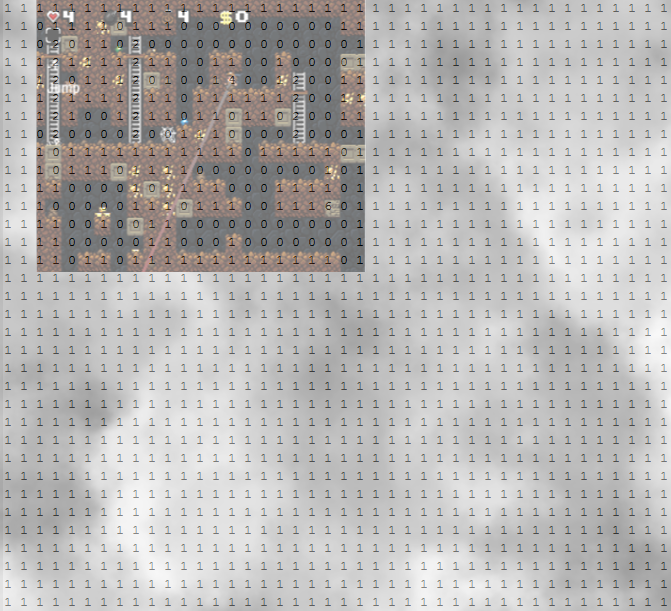
\includegraphics[width=.65\textwidth]{fig/spelunkbots-fow.png}
\caption {\label{fig:spelunkbots-fow}Visualização do sistema de \textit{fog of
war} demonstrando a diferença de informação recebida de elementos dentro e fora
do campo de visão do jogador.}
\end{figure}

\section{Utilização da \textit{API}}

É possível desenvolver \textit{bots} que fazem uso da \textit{API}
utilizando a linguagem GML (sigla para \textit{Game Maker Language}) ou
através da linguagem C++, ficando a critério do desenvolvedor a escolha da
linguagem. A única restrição que existe quanto ao uso de C++ dá-se no fato
de que a linguagem necessita de um processo de compilação através de uma
ferramenta externa, não sendo gerenciada diretamente pelo \textit{Game
Maker}. A figura \ref{fig:spelunkbots-usage-diagram} mostra a relação entre
o jogo, a \textit{API} e as possíveis linguagens de programação para se
utilizar. O código do Spelunky teve de ser modificado de forma a poder
interagir com o código do SpelunkyBots que, por sua vez, faz o uso de uma
solução de \textit{DLLs} escritas em C++ para fazer a interação com o jogo
através de código escrito em C++.

A \textit{API} permite uma interação completa com o jogo através do uso
das variáveis expostas pelo
\textit{framework}\footnote{http://spelunkbots.com/wp-content/uploads/2015/02/SpelunkBots-API-A-Getting-Started-Tutorial.pdf}.
Com elas, é possível fazer o controle da movimentação do bot, bem
como identificar o tipo de terreno em que se está pisando e os inimigos que
aparecem em seu campo de visão. Além disso, também são disponibilizadas
informações sobre as armadilhas que podem atrapalhar o jogador. Por fim,
existem variáveis que permitem um melhor controle das informações relativas ao
\textit{bot}, como o posicionamento no eixo X e no eixo Y, se o \textit{bot}
encontra-se virado para a esquerda ou para a direita, entre outros. O uso dessas
variáveis torna possível a implementação de técnicas de inteligência artificial
no jogo Spelunky. O apêndice \ref{appendix:spelunkbots-variables} faz um
detalhamento maior de todas essas variáveis.
